% Single side-view option B: slanted left outline; all 5 segments solid.
% Vertices E (bottom-left), L (top-left), B (top), R (bottom-right); diagonal E-B near left outline.
% Original "(B)" is the choice enumerator outside the geometry and is not redrawn.
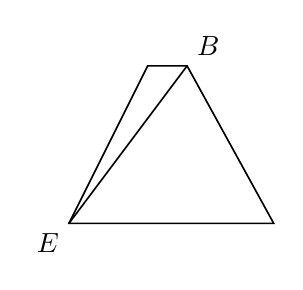
\begin{tikzpicture}[line width=.6pt,font=\normalsize,x=1cm,y=1cm]
\coordinate (E) at (0,0);
\coordinate (L) at (1.0,2);
\coordinate (B) at (1.5,2);
\coordinate (R) at (2.6,0);
\draw (E) -- (L) -- (B) -- (R) -- cycle;
\draw (E) -- (B);
\node[below left] at (E) {$E$};
\node[above right] at (B) {$B$};
\end{tikzpicture}
